\chapter{Introduction}

I am writing this introduction sitting in my living room in Kitchener, Ontario, staring at the dead ash tree which overlooks the empty lots bordering my home. Ash (\textit{Fraxinus sp.}) were a common group of trees planted along city streets in the eastern Unites States and Canada until the introduction of the emerald ash borer (\textit{Agrilus planipennis}, EAB) to North America in the 1990s \cite{nrcanmpb}. In the past two decades, the emerald ash borer (\textit{Agrilus planipennis}, EAB) has spread throughout the region, killing about 99\% of the ash trees in the regions they invade \cite{nrcaneab,herms2014emerald}. Once a prominent feature of deciduous woodlands in this area, \textit{Fraxinus} is now limited to rare pockets that have escaped the insect, and seedlings too small to be infested. This narrative is a familiar one. The American chestnut (\textit{Castanea dentata}) was once a major part of the carolinian forests, an important source of lumber and food. It was almost completely wiped out as the chestnut blight (\textit{Cryphonectria parasitica}) spread throughout eastern North America in the 19th and 20th centuries. Infectious agents in this way shape the landscapes we inhabit and the ecosystems we exist within. Of course, infectious agents are not limited to arboreal hosts: I have been in my living room staring at this dead ash tree for the past year, sheltering from the global COVID-19 pandemic. 

The various waves of the Black Death, the 1918 influenza pandemic, the HIV/AIDS pandemic, and the current COVID-19 pandemic, have irreversibly shaped our culture. Endemic infectious disease was a massive driving force in the formation of human societies everywhere until very recently. Only in the past century have some parts of the world been able to escape the spectre of endemic diseases such as malaria, polio, influenza, and measles, primarily through the invention of vaccination and understanding of disease spread dynamics. John Snow is considered to be one of the first epidemiologists, for his study of the spatial distribution of London Cholera outbreaks \cite{snow1855mode, brauer2019mathematical}, but the tools used in the field have evolved considerably since that time. Compartmental models have been one of the main tools used to forecast outcomes and mitigation strategies during recent outbreaks of infectious agents \cite{brauer2008compartmental}. Due to the ongoing pandemic, the general public is probably more aware than ever before of these models.

Compartmental models for the spread of infectious diseases are usually considered to have been introduced to the field by public health researchers, such as Hamer, Kermack, and McKendrick \cite{hamer1906epidemic, kermack1927contribution, brauer2019mathematical,edelstein2005mathematical}. This class of models divides the population into homogenous compartments, and describe the rate of movement between these compartments. The quintessential compartmental model is the SIR model (equations \ref{SIR}), so-called for its division of a population into susceptible (the $S(t)$ variable), infected (the $I(t)$ variable), and recovered (the $R(t)$ variable) compartments. 

\begin{eqnarray}
    \frac{dS}{dt} = -\beta S I  \\
    \frac{dI}{dt} = \beta S I - \gamma I\\
    \frac{dR}{dt} = \gamma I\\
    \label{SIR}
\end{eqnarray}

\begin{figure}
    \begin{minipage}[c]{0.4\textwidth}
    \centering
        \begin{tikzpicture}[node distance=1.5cm, auto,
            >=Latex, 
            every node/.append style={align=center},
            int/.style={draw, minimum size=0.5cm}]
        
        \node [int] (S)             {$S$};
        \node [int, right=of S ] (I) {$I$};
        \node [int, right=of I] (R) {$R$};
        \path[->] (S) edge node {$ \beta S I$} (I);
        \path[->] (I) edge node {$\gamma I$} (R);
        \end{tikzpicture}
        \caption{Diagram of population flow in an SIR model}
        \label{SIR_diagram}
    \end{minipage}\hfill
    \begin{minipage}[c]{0.55\textwidth}
        \centering
        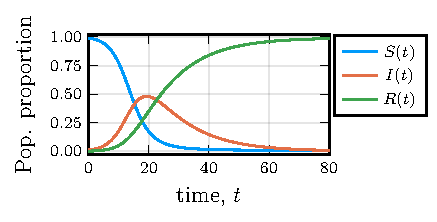
\includegraphics{chapter_0/sir.pdf}
        \caption{An infection represented by an SIR model, with $\beta = 0.4$, $\gamma = 0.08$, $S(0) = 0.99$, and $I(t) = 0.01$.}
        \label{SIR_plots}
    \end{minipage}
\end{figure}


The SIR model (Figures \ref{SIR_diagram},\ref{SIR_plots}) describes a population undergoing an infection that confers complete immunity after one has been infected, under a great number of simplifying assumptions: each compartment is totally homogenous, the probability that an individual recovers is constant per unit time, and the law of mass action. The law of mass action assumes that each individual in the $I$ compartment has a uniform probability $\beta$ of infecting any given individual in the $S$ compartment per unit time. It follows that for each $I$ individual, $\beta S$ people are expected to be infected per unit time, and therefore the total number of infections is expected to be $\beta S I$, which is the term removed from the $S$ compartment and added to the $I$ compartment. However, except during office icebreaker games, people do not mix homogeneously, so the assumption of homogeneity is a major drawback. Therefore, a common extension to this model is to add more structure, usually through further subdivision of the compartments \cite{hethcote2000mathematics}. For example, heterogeneity primarily dependent on population age can be represented by a chain of compartments \cite{hethcote1997age}. This idea can be also taken to its continuum limit yielding a system of hyperbolic partial differential equations \cite{anderson1985vaccination} which describe the evolution of a continuous age distribution. Spatial heterogeneity in host populations can be treated with reaction diffusion equations \cite{rass2003spatial}, but it can also be represented by systems of ordinary differential equations connected in a network, sometimes called a metapopulation model \cite{house2008deterministic,levins1969some,colizza2007invasion, nowzari2016analysis}. In contrast to a continuum of hosts distributed through space, this network formulation represents homogenously mixed groups that exchange hosts or infections with other homogenous groups. The popularity of this approach is probably due to their ability to easily represent different spatial topologies, and its resemblance to modern population patterns as tight communities of individuals connected by transport \cite{ball2015seven}. From the initial work on these models, the invention of computers and numerical integration methods have enabled researchers to get useful results from even the most complex elaborations on this theme. 

\section{Sars-CoV-2}

It is difficult to overstate the damage and loss of life that the ongoing COVID-19 pandemic has caused or exacerbated in the past year \cite{miller2020disease,who2021impact}. The first human case of Sars-CoV-2 occurred in late 2019 in central China, almost certainly transmitted from an animal host, very likely a bat \cite{andersen2020proximal,rasmussen2021origins,zhu2020novel}. The virus soon spread throughout the world, and was declared a pandemic by the World Health Organization (WHO), on March 11th, 2020 \cite{who2020announces}. Prior to the development, manufacture, and distribution of an effective vaccine, non-pharmaceutical interventions (NPIs) were the only option for control of the virus. We can distinguish two types of NPIs, scalable NPIs which require population participation (e.g. face masks, social distancing, hand washing) and those that do not (e.g.surface cleaning, increased ventilation). Compartmental models have been invaluable in modeling the spread of Sars-CoV-2 \cite{thompson2020epidemiological} and assessing the planning and efficacy of NPIs. Anderson et al. \cite{anderson2020estimating} use a compartmental model to assess efficacy of provincial lockdown restrictions on infection rates in British Columbia, Canada. They define two SEIR (Susceptible-Infected-Recovered-Exposed) models, one which corresponds to individuals using NPIs (primarily contact reduction), and another where NPIs are absent. Data from British Columbia, at least when the study was conceived, only contained the number of reported cases for each day, so the authors also include a stochastic model for estimating the delay from the actual case occurrence date to case report date. Fitting these models to the data they show that indeed, physical distancing policy was able to reduce the contact rate of people in British Columbia, more than was necessary to push $R$ below 1. In the months prior to widespread immunization, people around the world endured various levels of NPI policy. Government policy on NPIs has ranged from comprehensive quarantine procedures (in e.g. New Zealand, South Korea, Singapore, Vietnam) to almost nothing at all (e.g. some of the United States, Sweden, Brazil). In the outcomes of the aforementioned countries, empirical research, and modelling studies, NPIs have been shown to be an effective method for the control of COVID-19 \cite{flaxman2020estimating,ferguson2020report,demirguc2020sooner}. 

\section{Imitation dynamics}

The demonstrated effectiveness of NPIs implies that the immense morbidity and mortality over the past year is not simply a natural disaster but a humanitarian one. Since our survival depends on our ability to construct a world in which people are incentivized to centre the well-being of others, any attempt to model human outcomes of the pandemic should also attempt to model the incentive structures we operate within. Game theory provides a simple, but effective framework for many of the aforementioned systems \cite{andrews2015disease,jentsch2018spatial}. In a game theoretical sense, scalable NPI usage can be viewed as a prisoners dilemma in that everyone either cooperates or defects with the practice of using certain NPIs, and the decision to defect or to cooperate is based on a combination of the perceived payoff to do so, and the influence of the rest of the population \cite{reluga2010game}. Table \ref{prisonersdilemma} shows the payoff matrix of this 2-player game. Of course in real life, we are all playing this game, all the time, with everyone. 
\begin{figure}
    \centering
    \begin{tabular}{ |c|c| c| } \hline
        \diagbox[width = 7em, height = 2em]{P1}{P2} &use NPI& don't use NPI   \\ \hline
        use NPI & \diagbox[width = 13em, height = 8em]{low risk,\\ NPIs unpleasant}{low risk,\\ NPIs unpleasant} &  \diagbox[width = 13em, height = 8em]{med risk,\\ NPIs unpleasant} {med risk}\\ \hline 
        don't use NPI & \diagbox[width = 13em, height = 8em]{med risk}{med risk,\\ NPIs unpleasant} &  \diagbox[width = 13em, height = 8em]{high risk}{high risk}   \\ \hline
    \end{tabular}
    \caption{NPI adoption as a two-player game (between P1 and P2).}
    \label{prisonersdilemma}
\end{figure}


The simplest way to approximate the time evolution of a such a game is with the one-dimensional replicator equation, which approximates these dynamics in terms of the population average \cite{hofbauer1998evolutionary}. Specifically, we introduce a variable $x(t)$ which represents the proportion of people adopting a strategy, then the replicator equation \ref{replicator} gives the time-evolution of $x(t)$ in terms of the payoff for cooperating over defecting, $p(x,t)$. We see immediately that this equation, disregarding $p(x,t) = 0$, has two steady states: $x = 1$ and $x = 0$. Given $p(x,t)$ constant, the population will approach whichever point it is initially closer to. 

\begin{equation}
    \frac{dx}{dt} = \sigma x(1 - x)p(x,t) 
    \label{replicator}
\end{equation}


This formulation has been also used to model vaccination sentiment in a variety of scenarios \cite{oraby2014influence,bauch2004vaccination,bauch2005imitation,bauch2012evolutionary}. In this context, ``cooperation" refers to the strategy of getting a widely-available vaccine, and the cooperation payoff function is usually of the form in equation \ref{vacpayoff}. The population is assumed to have a constant payoff to avoid vaccination (in many cases, just due to inconvenience) and a payoff to vaccinate proportional to $I$, the prevalence of infection in the model. 

\begin{equation}
    p(x,t) = - c + \rho I
    \label{vacpayoff}
\end{equation}


A prisoner's dilemma formulation and model based upon equation \ref{replicator} coupled to an application-specific model (in the above case, disease dynamics), can also be applied to human-environment models in ecology. In particular, it has been used to model conservation responses coupled to ecosystem dynamics in contexts such as forest-grassland mosaics \cite{innes2013impact,henderson2016alternative}, global climate \cite{bury2019charting}, coral reefs \cite{thampi2018socio}, agricultural land use \cite{gooding2018forest}. I will focus on the application of imitation dynamics to forest pest transport, and the use of NPIs in the context of the COVID-19 pandemic.


\section{Forest pests in eastern North America}
The term ``forest pests" covers a broad range of infectious agents that are responsible for forest tree damage and mortality. Major invading forest pests in eastern North America include: the Asian longhorned beetle (\textit{Anoplophora glabripennis}), the butternut canker (\textit{Ophiognomonia clavigignenti-juglandacearum}), \textit{Lymantria dispar dispar}, dutch elm disease \textit{Ophiostoma ulmi}, and the aforementioned EAB (Figure \ref{eabfig}). Together, these non-native pests kill 5.53 teragrams of carbon worth of trees each year, on an order of magnitude comparable to forest fires in North America \cite{fei2019biomass}. Non-native insect invaders are usually introduced by accident. The majority of recently introduced species are a result of careless global trade, with new individuals arriving in lumber, live plants, or similar goods \cite{brockerhoff2017ecology}. Models for the spread of these insects are often inspired by models for infectious diseases in humans. Research in mathematical ecology generally uses the related Lotka-Volterra model for host-parasitoid dynamics \cite{edelstein2005mathematical}, but SIR models can be a natural choice because they focus on the time-evolution of the host populations, which is often the more useful quantity \cite{edelstein2005mathematical}. 

Barlow et al. \cite{barlow2014modelling} couple a compartmental model of an invading forest pest to human travel patterns. Humans have been shown to be a common vector for forest pests \cite{buck2009hitchhiking,kolar2001progress,wilson2009something}, so our effect on the long-distance spread of forest pests is important to understand. They assume that forests occur as homogenously mixed patches, each with its own compartmental dynamics. Transport between each patch is assumed to be proportional to local sentiment towards firewood transport. Their model for human travel behavior uses imitation dynamics, where the payoff for travel is a function of the price of firewood and the perceived level of pest infestation in a patch. Barlow et al. show that, at least with a small number of patches, lowering the cost of firewood is generally effective at reducing equilibrium infestation. Education on the risk of firewood transport, corresponding to an increase the level of concern for infestation levels in a local patch, can also be effective in their model. They find that a drawback of education as a tactic is that resilience to pest reintroduction is low, because transport behavior returns to normal after pests populations have dropped. In chapter \ref{ch2} we extend their model to a realistic transport network, and include pest mitigation strategies that explicitly use the spatial heterogeneity in the model.  


\begin{figure}
    \begin{minipage}[c]{0.45\textwidth}    
        \centering
        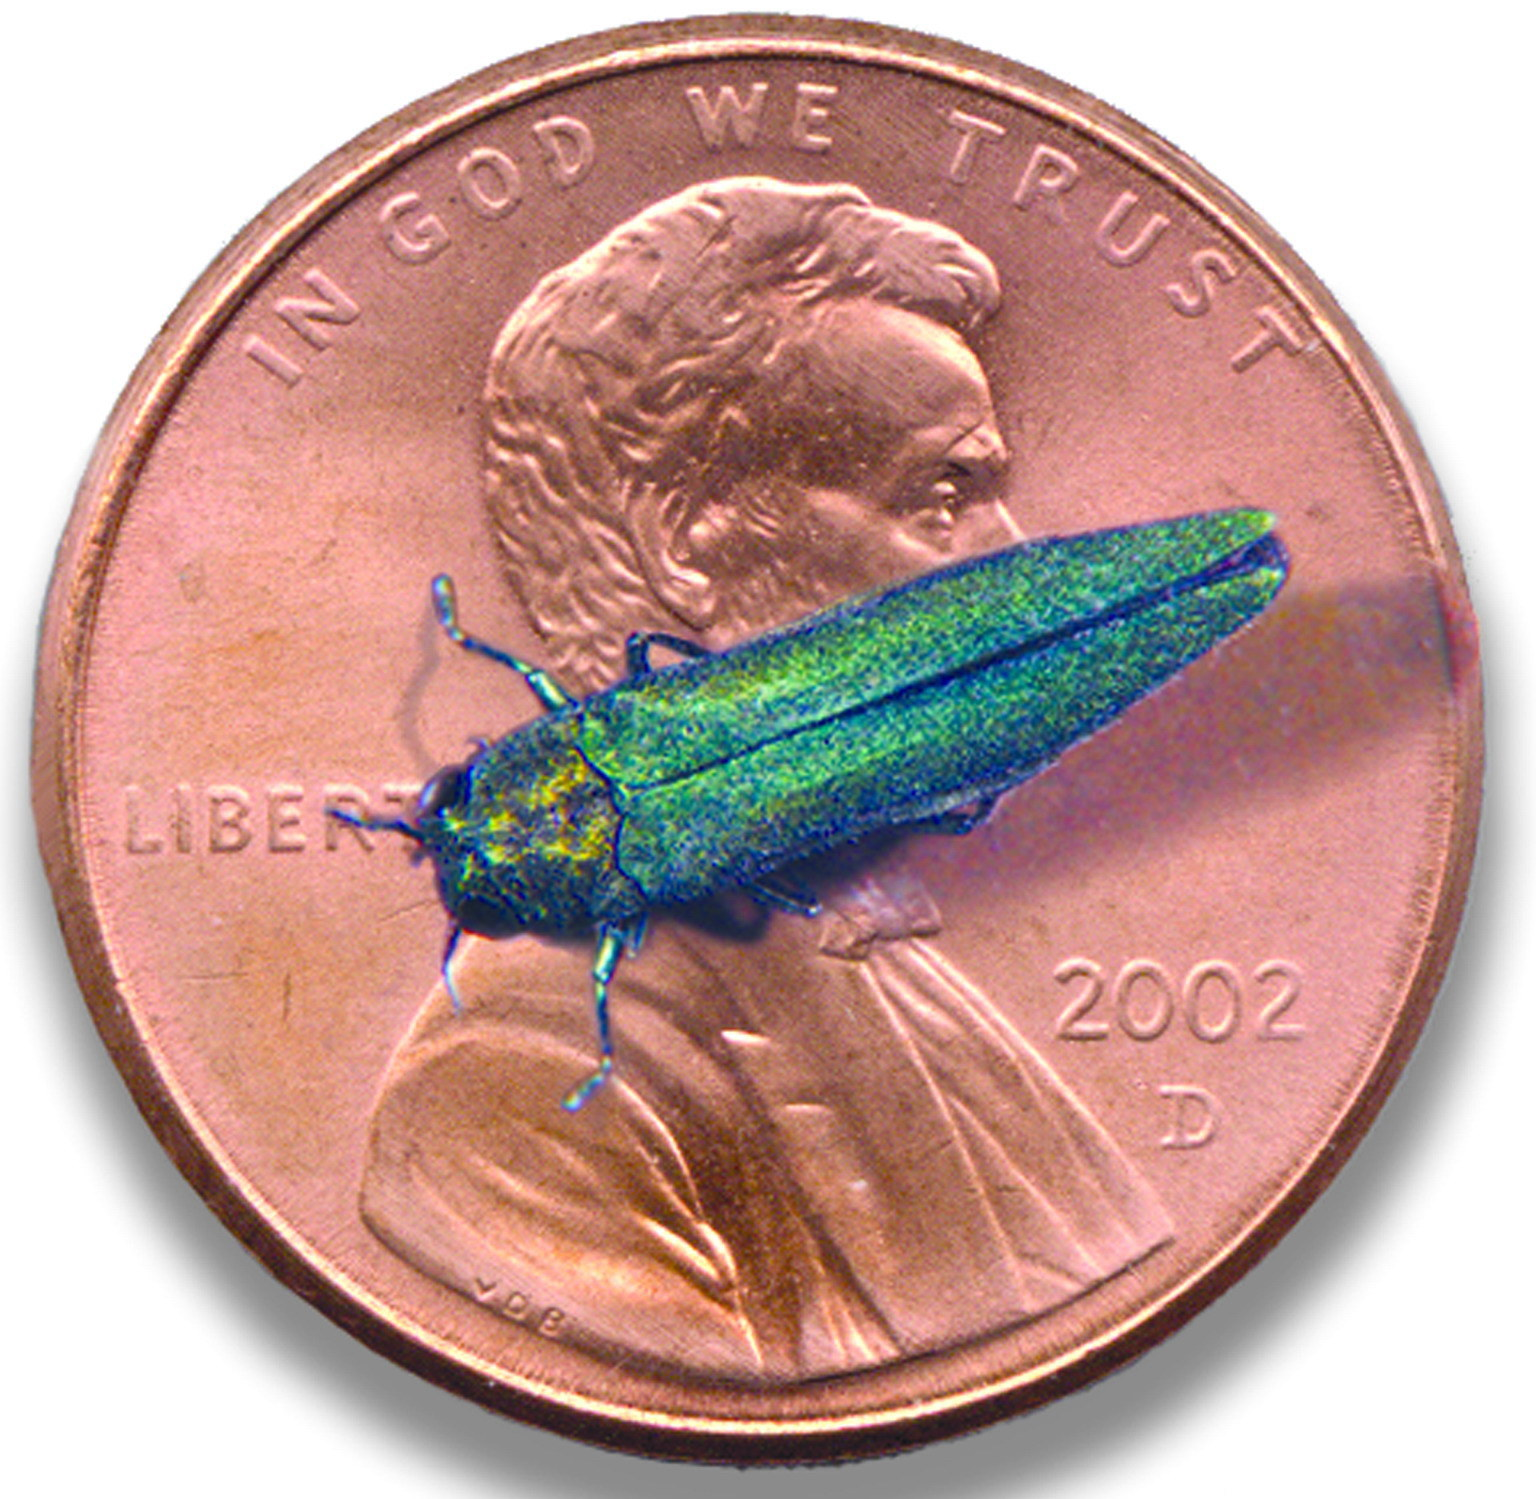
\includegraphics[width=\textwidth]{chapter_0/Emerald_ash_borer_penny.jpg}
        \caption{An EAB on a penny \cite{eab_penny_photo}}
        \label{eabfig}
    \end{minipage}\hfill
    \begin{minipage}{0.45\textwidth} 
        \centering
        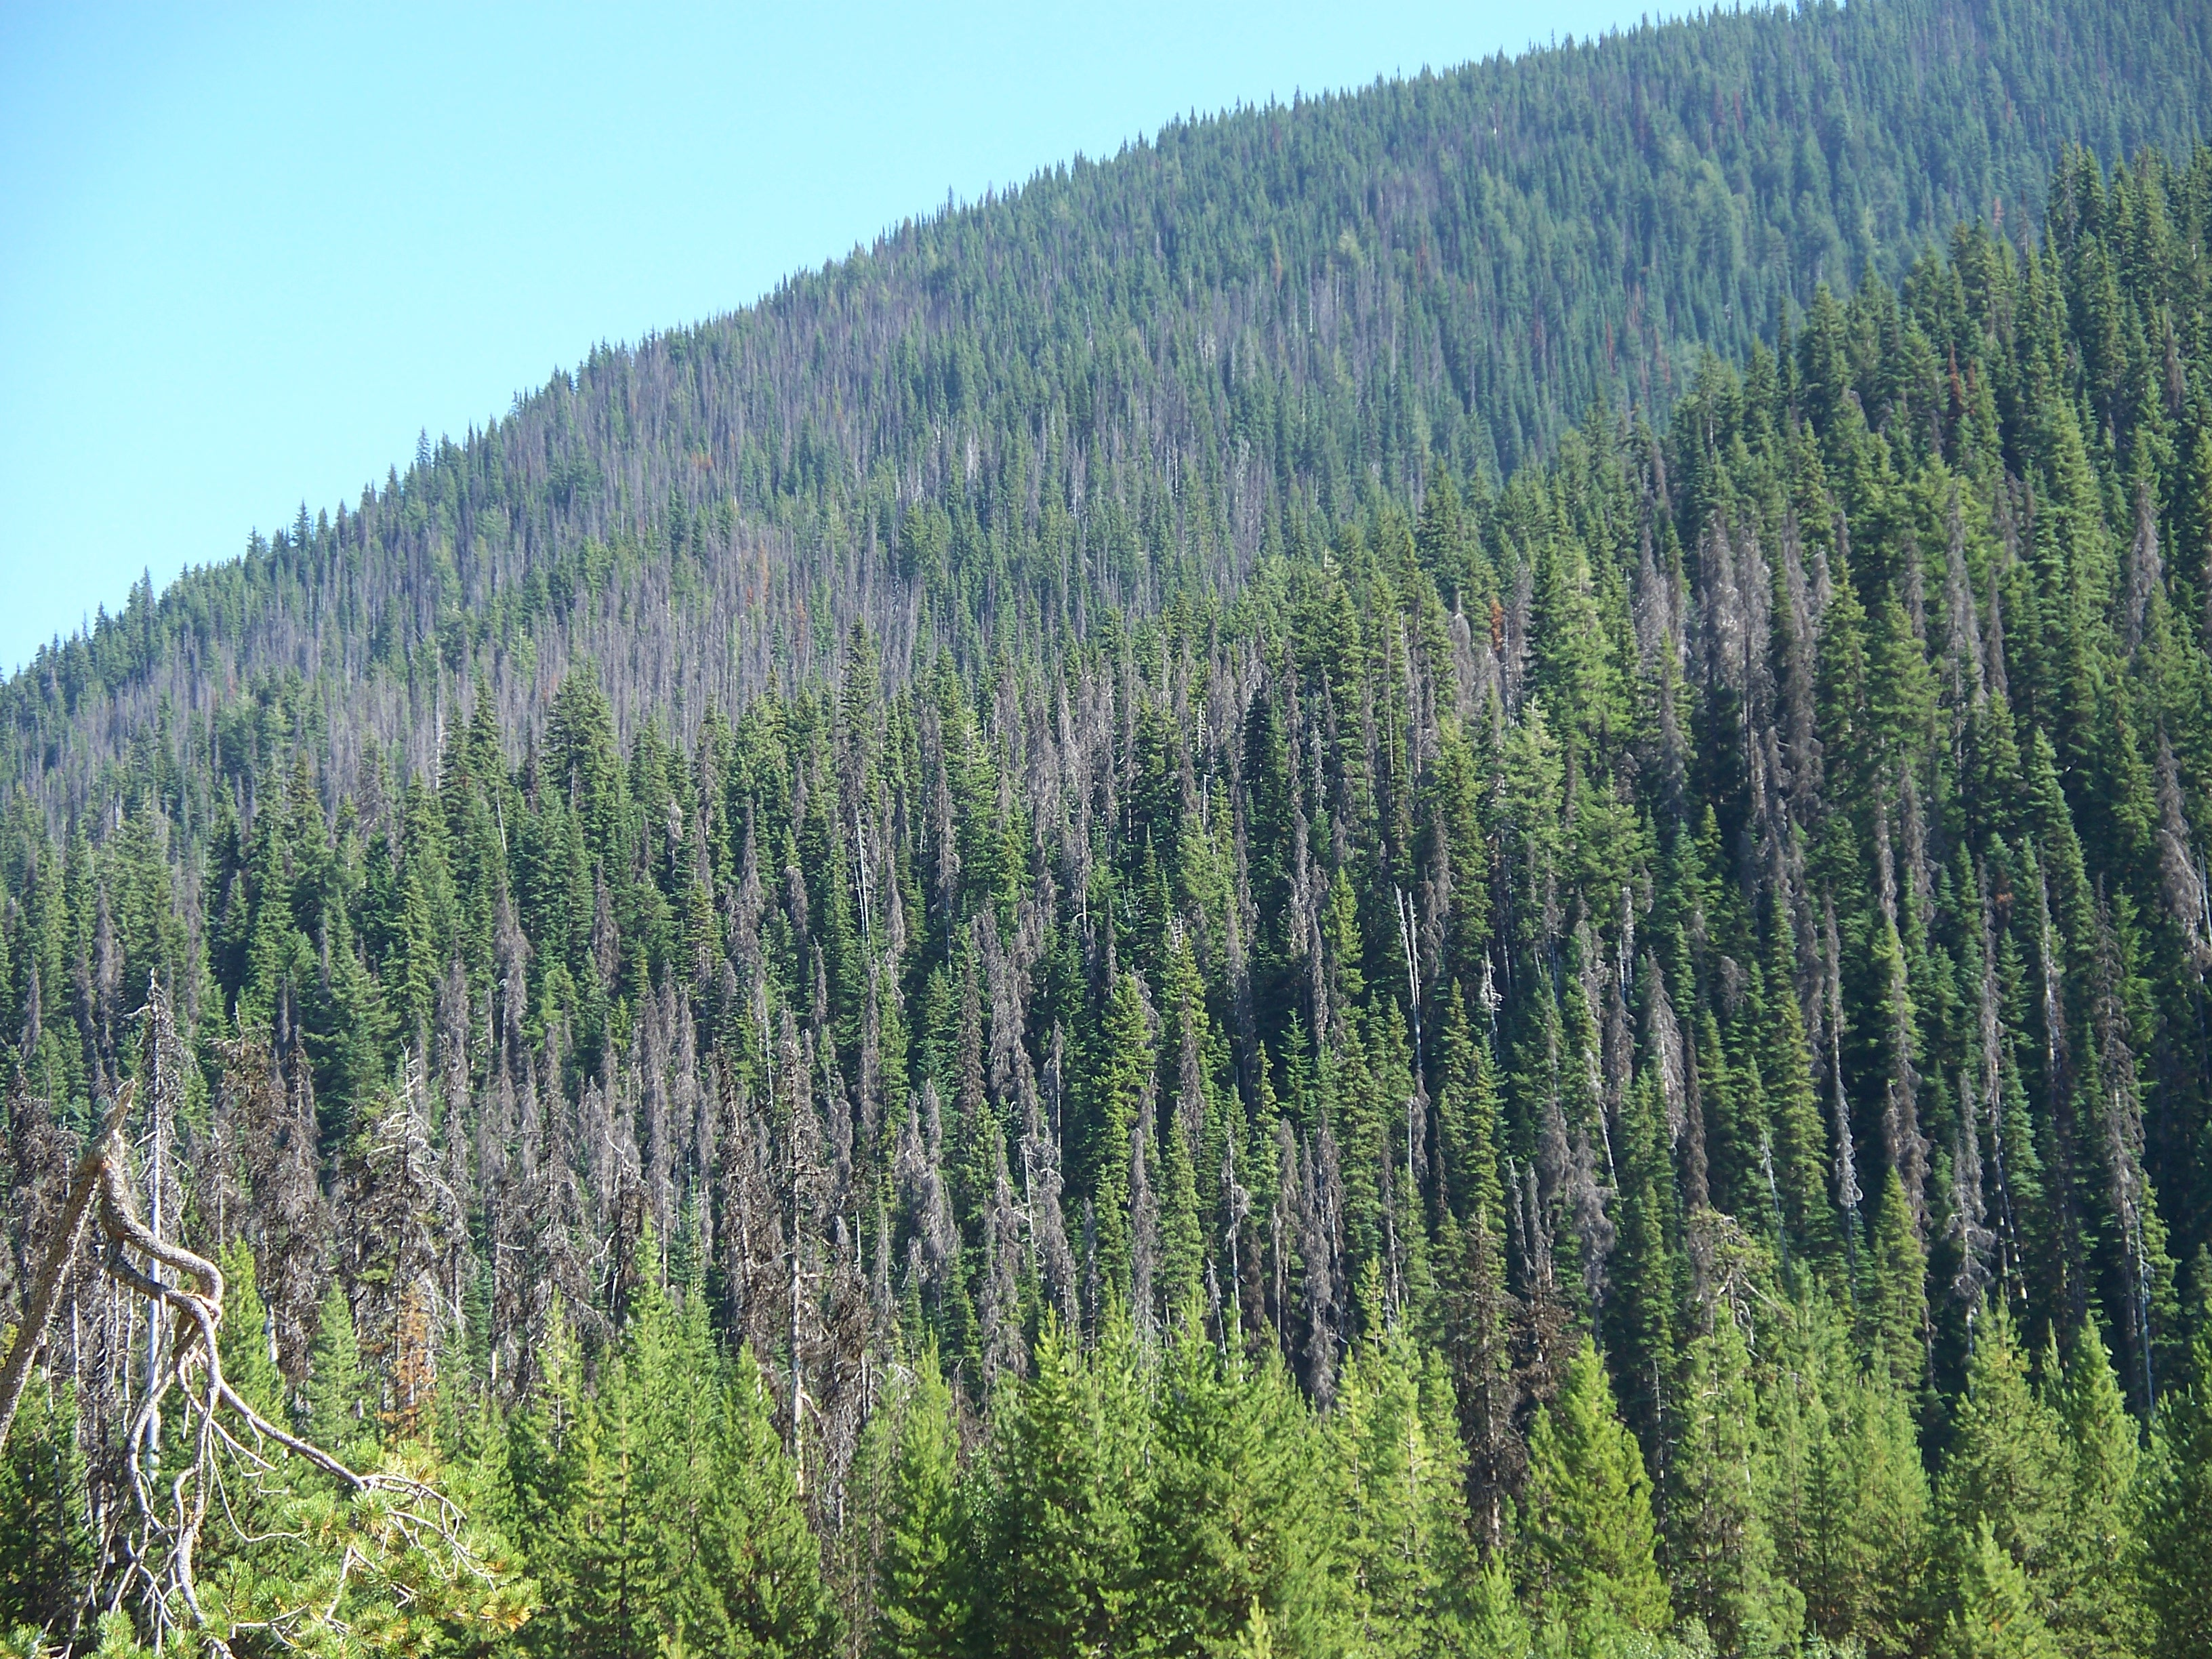
\includegraphics[width=\textwidth]{chapter_0/Pine_Beetle_in_Manning_Park.jpg}
        \caption{MPB-killed lodgepole pines in Manning Park, British Columbia, Canada \cite{mpb_manning_park}}
        \label{mpbfig}
    \end{minipage}
\end{figure}

\section{Mountain pine beetle (MPB) and fire-driven forest ecosystems of the Western Cordillera}


The coniferous forests of the western cordillera of North America are the subject of the model presented in chapter \ref{ch3}. The Canadian section of these forests are primarily composed of a mixture of \textit {Pinus} sp., namely lodgepole pine (\textit{Pinus Contorta}), but also ponderosa pine (\textit{Pinus ponderosa}) \cite{brown2010impact}. The fire regimes in these forests are generally characterized by frequent, low to mixed severity fires depending on elevation and climactic conditions \cite{agee1996fire,arno1980forest}. In these regions, there are also a few other dominant forest types: those dominated by Douglas Fir (\textit{Pseudotsuga menziesii}), and those dominated by subalpine spruce (\textit{Abies lasiocarpa}). These other forest types become dominant in areas which experience wetter or cooler climates, as they are less drought tolerant, and also less fire resistant \cite{JENKINS200816}. Therefore, the lodgepole pine forests are dependent on a frequent fire regime to maintain climax lodgepole forests. They are very rapidly growing when young, possess (usually) serotinous cones, and maintain massive seed banks in the soil to rapidly colonize the area after disturbances \cite{lotan1976cone,lotan1985role}.

Besides wildfire, MPB (\textit{Dendroctonus ponderosae}) is the most significant disturbance in these forest types. Endemic to this ecosystem, MPB most commonly attacks lodgepole pine in Canada \cite{safranyik2007mountain} (Figure \ref{mpbfig}), but it can attack and reproduce within all of the pine species in North America, and during outbreaks has been recorded to attack spruce and fir trees within its range \cite{gibson2009mountain}. MPB, and bark beetles more generally, exhibit highly cyclic lifestyles. For most of the year, they exist in the phloem of the tree first as eggs, then as larvae, until they are mature enough to emerge and fly to new hosts. The emergence of MPB occurs in late summer, although it is heavily dependent on the climate that year \cite{bentz2014mountain}. While their flight capability is limited, MPB can use air currents to colonize trees over 20km away from their place of birth \cite{shegelski2019morphological}. When individuals find a suitable host, they release pheromones that attract other flying beetles and triggering a mass attack behaviour. This behaviour functions to overwhelm the defenses of the host tree. A successful attack results in the MPB laying their eggs in the phloem of the new host tree, and the cycle repeats. Older trees with thicker phloem are most susceptible to MPB attack, and they are generally the first to be colonized, with MPB attacking progressively less suitable hosts as population densities rise \cite{safranyik2007mountain}. Endemic periods of low MPB density give rise to outbreaks based on a variety of factors, such as density of good hosts, climate, and possibly wildfire damage \cite{safranyik2007mountain}. Although MPB has always exhibited outbreak cycles, in the past two decades, outbreak sizes have exceeded historically recorded levels probably due to increases in winter temperatures and higher densities of mature trees \cite{bentz2010climate,safranyik2007mountain}. Recently, jack pine \textit{Pinus banksiana} stands in northern Alberta, and the Northwest Territories, have been attacked by MPB as they expand their range north and eastward \cite{cudmore2010climate,nrcanmpb}. Understanding the holistic dynamics of these ecosystems, and the role that MPB takes within them, will be key to understanding the causes and effects of these unprecedented population levels. 

An early model of bark beetle (a larger group to which MPB belongs) dynamics is that of Berryman et al. \cite{berryman1984metastability}. Their model is not a compartmental one, rather they explicitly represent tree (host) and MPB (pathogen) populations. It is assumed that trees $T(t)$ exhibit logistic growth up to a constant carrying capacity, and die according to a function $g(T(t),B(t))$ where $B(t)$ is the population of bark beetles at time $t$. Bark beetles also exhibit logistic growth, but their carrying capacity is proportional to by $g(T,B)$. The crux of this model is therefore the shape of the function $g$. This function exhibits a threshold in $T$ that decreases as the beetle population $B$ increases, describing the ability for outbreak bark beetle populations to more easily overcome defenses of vigorous trees. They conclude from this model that thinning forest stands is useful to maintain resilience to bark beetle outbreaks. Their approach is reflected in a more recent model by Lewis et al \cite{lewis2010structured}, which extends the idea to an integral project model that explicitly represents the vigor distribution of the stand, and its effect on beetle reproduction. 

Mechanistic population models are widespread in bark beetle dynamics, but most wildfire modelling has a distinctly different flavour. In the past few decades, the field has largely converged to physics based models which explicitly represent combustion chemistry, forest geography, and atmospheric fluid dynamics \cite{linn2002studying,mell2007physics,bakhshaii2019review}. This comes from a need to produce detailed forecasts on the precise extent, severity, and velocity of wildfires, often in real time. There are some examples of compartmental-style models explicitly modeling wildfires \cite{casagrandi1999minimal}, but when they are coupled to forest pests often fire is modeling implicitly \cite{chen2014model}.

\section{Thesis Outline}

In the first chapter, an age-structured impulsive differential equation model of COVID-19 is coupled to the aforementioned imitation dynamics for physical distancing. It is parameterized with case data from Ontario, Canada and population location data from Google. Two primary categories of vaccination strategy were considered in this model: vaccination of the most vulnerable populations (older age groups), or vaccination of the most transmitting populations (according to contact distribution estimates). We analyze how the timing, supply rate, and shutdown policies will affect the best vaccination policy through numerical simulation of the model.

The second chapter extends the forest pest and firewood transport model of Barlow et al. \cite{barlow2014modelling} to a large empirically derived network of human movement patterns between susceptible forest patches. Numerical analysis of this model is done to compare the effectiveness of three major policy categories in reducing the spread of invasive pests throughout forested areas in Eastern Canada. We consider direct interception of human-mediated transport of forest pests, changing behavioural incentives to transport firewood, and quarantine of the most central areas, and combinations thereof. These strategies are assessed with respect to total tree infections over periods of 5, 10, and 20 years.

The third chapter extends an age-structured, discrete time model of mountain pine beetle population \cite{duncan2015model} to include a simplified model of yearly burn sizes. The effect of changing fire disturbance regimes on the forest stand structure is explored through numerical simulations of the parameter space. Since MPB outbreak patterns seem to strongly depend on the density of mature trees, they are therefore sensitive to stand structure, in particular the creation of large-even aged stands created by severe forest fires. We discuss the dynamical regimes of this system, and argue that outbreak dynamics can be significantly influenced by heterogeneity in stand structure. The final chapter will summarize and contextualize these results, discuss their limitations, and outline opportunities for future work.

Each chapter studies a coupled compartmental model specialized to a particular domain. We compare various mitigation strategies such vaccine prioritization for Sars-CoV-2, and forest stand thinning in out MPB-wildfire model. Counterfactuals are used to determine the most effective mitigation strategies for each system.  The three chapters are followed by a synthesis and summary of the results from each chapter, and discussion of their limitations and the opportunities for future work. 